\definecolor{exxetagray}{gray}{0.75}
\definecolor{itemcolor}{RGB}{179,217,255}
\definecolor{usercolor}{RGB}{255,204,179}

\shorthandoff{"}
\chapter{Diskussion}
\label{ch:diskussion}

\section{Zusammenfassung der Ergebnisse}
Im Rahmen der quantitativen Forschung dieser Arbeit wurde untersucht, ob der multi-kriterielle Ansatz für die Berücksichtigung der bilateralen Präferenzen robust die Zufriedenheit von Mitarbeitern sowie deren erwartete Arbeitsleistung aus Sicht der Manager bei der Besetzung von offenen Projektpositionen erhöhen kann.
Anhand einer Befragung unter den Mitarbeitern des IT-Unternehmens EXXETA wurden Fähigkeiten und Präferenzen von Mitarbeitern sowie deren Zufriedenheit mit ausgewählten Beispielprojekten ermittelt.
Eine Befragung unter den Managern desselbigen Unternehmens diente dazu, die zu erwartende Arbeitsleistung der befragten Angestellten in den ausgewählten Projekten zu bestimmen.
Die Zufriedenheit und die zu erwartende Arbeitsleistung wurde jeweils für die empfohlenen Mitarbeiter des unilateralen sowie die empfohlenen Mitarbeiter des bilateralen Ansatzes gemessen und miteinander verglichen.
Insgesamt konnte festgestellt werden, dass der bilaterale Algorithmus im Mittel in vier von fünf Projekten eine höhere Zufriedenheit erzielte und in einem der fünf Projekte eine Steigerung der Arbeitsleistung bewirkte.
Dabei führte der bilaterale Algorithmus in 28 Prozent der Fälle zu einer erhöhten Zufriedenheit unter den empfohlenen Mitarbeitern und in 20 Prozent der Fällen zu einer Steigerung der prognostizierten Arbeitsleistung der empfohlenen Angestellten.
Zugleich führte der bilaterale Algorithmus in 12 Prozent der Fälle zu einer Verschlechterung der erwarteten Arbeitsleistung.
Der Rückgang der Arbeitsleistung konnte zwei der fünf Projekte zugeordnet werden.
Lediglich in 8 Prozent der Fälle bewirkte der bilaterale Algorithmus einen Rückgang der Zufriedenheit unter den empfohlenen Mitarbeitern.
Die Verschlechterung der Zufriedenheit wurde genau in einem der fünf Projekte bewirkt.
% In 12 Prozent der Fälle führte der bilaterale Algorithmus dagegen zu einer Verschlechterung der zu erwartenden Arbeitsleistung.
% In 8 Prozent der Fälle bewirkte der bilaterale Algorithmus sogar eine Verschlechterung der Zufriedenheit unter den empfohlenen Mitarbeitenden.

% Kurz eingehen auf die ergebnisse der präferenz und fähigkeitsbefragung
Bei der Befragung der Mitarbeiter zu ihren Fähigkeiten und Präferenzen konnte festgestellt werden, dass Mitarbeiter den Großteil der angefragten Fähigkeiten präferierten, während sie nahezu gleich vielen angeforderten Fähigkeiten neutral gegenüber standen.
Weiter wurde sichtbar, dass ein Großteil der präferierten Fähigkeiten von Mitarbeitern zugleich beherrscht wurde.
Durch die Integration der negativen Präferenzen wurde sichtbar, dass Mitarbeiter bei über 22 Prozent der angeforderten Fähigkeiten kein Interesse zeigten diese in zukünftigen Projekten einsetzen zu wollen.
Ein Vergleich der Erfüllung der Präferenzen der Mitarbeiter durch die angeforderten Projektpositionen und deren Zufriedenheit in den jeweiligen Projekten zeigte darüber hinaus bei zwei der fünf Beispielprojekte eine auffällige Diskrepanz.

Die Befragung der Manager legte offen, dass deren Angaben zu der prognostizierten Arbeitsleistung der Mitarbeiter in den ausgewählten Projekten bei zwei der Beispielprojekte auffällig auseinanderfielen. 
Ein Vergleich der Erfüllung der angeforderten Projektpositionen durch die Mitarbeiter und deren erwarteter Arbeitsleistung nach Angaben der Manager zeigte darüber hinaus, dass die angegebenen Angestellten in einigen Projekten nicht konkruent mit den Mitarbeitern mit der höchsten Erfüllung der angeforderten Projektpositionen waren.

Abschließend wurde betrachet, wie sich die Gewichtung von Fähigkeiten und Präferenzen auf die Zufriedenheit und die Arbeitsleistung der Mitarbeiter auswirkte.
Dabei wurde festgestellt, dass die Methode zur Bestimmung des optimalen Gewichts bei unterschiedlichen Kombinationen der Traningsdatensätze zu Gewichten führte, die alle in einen Bereich zwischen 0.6 und 0.8 fielen.
Bei Betrachtung der Zufriedenheit und der Arbeitsleistung unter Anwendung der verschiedenen Gewichte fiel auf, dass die Verbesserung in der Zufriedenheit und der Arbeitsleistung durch kein bestimmtes Gewicht erzielt wurde.
Auch die Fälle, die eine Verschlechterung der Zufriedenheit bzw. der Arbeitsleistung aufwiesen, konnten nicht gezielt einem Gewicht zugeordnet werden.

\section{Interpretation der Ergebnisse}
Basierend auf den Forschungsergebnissen von \textcite[S.1 ff.]{link:booklet} wurde die Annahme aufgestellt, dass ein alternativer Ansatz für die Berücksichtigung der Präferenzen beider Parteien in einem bilateralen Empfehlungssystems robust zu einer verbesserten Zuordnung von Person zu Umgebung im Vergleich zu einem unilateralen System führen kann.
% Als Indikatoren einer optimalen Zuordnung betrachtete \textcite[S.1 ff.]{link:booklet} die Kennzahlen Zufriedenheit und Arbeitsleistung.
Die Ergebnisse der quantitativen Forschung zeigen, dass der entwickelte multi-kriterielle Ansatz für das bilaterale Empfehlungssystem verglichen mit dem unilateralen System in vier von fünf Projekten im Mittel eine höhere Zufriedenheit unter den empfohlenen Mitarbeitern erzielen konnte (Vgl. Abbildung \ref{fig:ergebnisse:abb8}).
Zugleich blieb die Arbeitsleistung in vier von fünf Projekten im Mittel konstant, wobei in einem der fünf Projekte im Durchschnitt sogar eine Steigerung der Arbeitsleistung unter Einsatz des bilateralen Algorithmus erzielt wurde (Vgl. Abbildung \ref{fig:ergebnisse:abb10}).
Insgesamt lassen die Auswirkungen des entwickelten bilateralen Algorithmus auf die durchschnittliche Zufriedenheit und Arbeitsleistung der Mitarbeiter daher die Vermutung zu, dass eine Berücksichtigung der Präferenzen grundsätzlich vorteilhaft ist.

Entgegen der Erwartungen bewirkte der bilaterale Algorithmus in zwei von 25 Fällen eine Verschlechterung der Zufriedenheit unter den empfohlenen Angestellten (Vgl. Abbildung \ref{fig:ergebnisse:abb9}).
Ein Vergleich der unilateralen und bilateralen Rankings zeigte, dass die Verschlechterung der Zufriedenheit in beiden Fällen durch denselben Mitarbeiter in Projekt 3 bewirkt wurde.
Tabelle \ref{tab:diskussion:tab1} stellt für einen der Fälle ($\alpha$ = 0.6068) das unilaterale Top-5-Ranking im Vergleich zu den Rängen der Mitarbeiter im bilateralen Ranking dar.
Aus Datenschutzgründen wurden die Mitarbeiter in der Tabelle pseudonymisiert.

\begin{table}[htbp]
    \begin{center}
    \begin{tabular}{c|p{0.7in}|p{0.95in}|p{0.7in}|p{0.95in}}
    {\textbf{Mitarbeiter}} & {\textbf{Rang unilateral}} & {\textbf{Präferenzwert unilateral}} & {\textbf{Rang bilateral}} & {\textbf{Präferenzwert bilateral}} \\
    \hline
	Mitarbeiter A & \hfil1 & \hfil0.625 & \hfil3 & \hfil0.5759 \\
    \hline
    Mitarbeiter B & \hfil2 & \hfil0.625 & \hfil5 & \hfil0.5513 \\
    \hline
	Mitarbeiter C & \hfil3 & \hfil0.625 & \hfil6 & \hfil0.5514 \\
    \hline
	Mitarbeiter D & \hfil4 & \hfil0.625 & \hfil2 & \hfil0.6004 \\
    \hline
	Mitarbeiter E & \hfil5 & \hfil0.5625 & \hfil1 & \hfil0.6362 \\
    \end{tabular}
    \end{center}
    \caption[Vergleich des unilateralen Top-5-Rankings mit den bilateralen Rängen der empfohlenen Mitarbeiter für Projekt 3 ($\alpha$ = 0.6068)]{Vergleich des unilateralen Top-5-Rankings mit den bilateralen Rängen der empfohlenen Mitarbeiter für Projekt 3 ($\alpha$ = 0.6068)}
	\label{tab:diskussion:tab1}
\end{table}

Daran ist zu erkennen, dass der Mitarbeiter C durch die Berücksichtigung der Präferenzen im bilateralen Ranking auf Rang 6 platziert wurde und damit nicht mehr unter die fünf empfohlenen Mitarbeiter fiel.
% Der Mitarbeiter wurde aufgrund seiner geringen Übereinstimmung der angegebenen Präferenzen mit den angeforderten Projektpositionen von Projekt 3 im bilateralen Ranking niedriger platziert als im unilateralen Ranking.
Obwohl der Mitarbeiter die Mehrheit der angeforderten Fähigkeiten des Projekts nicht präferierte, konnte festgestellt werden, dass dieser in der Befragung dennoch angab mit dem Projekt grundsätzlich zufrieden zu sein.
Die geringere Zufriedenheit bei bilateraler Empfehlung wurde folglich durch eine niedrigere Platzierung des Mitarbeiters aufgrund der hohen Gewichtung der Präferenzen im Vergleich zum unilateralen Ranking bewirkt.
Der Sachverhalt lässt vermuten, dass neben den Präferenzen eines Mitarbeiters offenbar weitere unbekannte Faktoren existieren, die die Zufriedenheit eines Angestellten beeinflussen.
Eine mögliche Erklärung hierfür liefert die Theorie von \textcite[S. 1ff.]{malinowski:2006}, welche besagt, dass die Zuordnung von Person zu Arbeitsumgebung (\ac{P-E Fit}) von mehreren Faktoren beeinflusst wird.
Neben den Bedürfnissen der Person nennen \textcite[S. 1ff.]{malinowski:2006} unter anderem die Teamzugehörigkeit (Person-Group-Fit).
Eine weitere Annahme ist, dass unterschiedliche Fähigkeiten in Projekten von unterschiedlicher Bedeutung für einen Mitarbeiter sind.
Es wird vermutet, dass das Vorhandensein oder Fehlen bestimmter Projektposition in einem Projekt ausschlaggebend für die Zufriedenheit eines Mitarbeiters in einem Projekt sein kann, unabhängig von dessen übrigen Präferenzangaben.

Hinsichtlich des Verhaltens der beiden Kriterien (Präferenzerfüllung Manager, Präferenzerfüllung Mitarbeiter) wurde angenommen, dass die Berücksichtigung der Präferenzen der Mitarbeiter bei der Zuordnung zu Projekten mit deren beherrschten Fähigkeiten, welche in die Präferenzerfüllung der Manager einfliessen, in Konkurrenz stehen kann.
% Ein solches Verhaltenzwischen den Zielvorstellungen stellten unter anderem \textcite[S. 12]{rodriguez:inproceedings} in ihrer Forschung zu fest.
Es wurde daher durchaus erwartet, dass eine Berücksichtigung der Präferenzen der Mitarbeiter in einigen Fällen auch zu einer Reduktion der erwarteten Arbeitsleistung führen würde.
Die absolute Veränderung der Arbeitsleistung der Mitarbeiter von unilateralem zu bilateralem Algorithmus nach Projekt in Abbildung \ref{fig:ergebnisse:abb11} zeigte, dass dies in drei von 25 Fällen auftrat.
Tabelle \ref{tab:diskussion:tab2} stellt für einen der Fälle (Projekt 2, $\alpha$ = 0.6068) das unilaterale Top-6-Ranking im Vergleich zu den Rängen der Angestellten im bilateralen Ranking dar.
Aus Datenschutzgründen wurden die Mitarbeiter in der Tabelle pseudonymisiert.

\begin{table}[htbp]
    \begin{center}
    \begin{tabular}{c|p{0.7in}|p{0.95in}|p{0.7in}|p{0.95in}}
    {\textbf{Mitarbeiter}} & {\textbf{Rang unilateral}} & {\textbf{Präferenzwert unilateral}} & {\textbf{Rang bilateral}} & {\textbf{Präferenzwert bilateral}} \\
    \hline
	Mitarbeiter A & \hfil1 & \hfil0.875 & \hfil3 & \hfil0.7767 \\
    \hline
    Mitarbeiter B & \hfil2 & \hfil0.8125 & \hfil1 & \hfil0.8862 \\
    \hline
	Mitarbeiter C & \hfil3 & \hfil0.75 & \hfil2 & \hfil0.7992 \\
    \hline
	Mitarbeiter D & \hfil4 & \hfil0.5 & \hfil4 & \hfil0.6720 \\
    \hline
	Mitarbeiter E & \hfil5 & \hfil0.375 & \hfil6 & \hfil0.4979 \\
    \hline
	Mitarbeiter F & \hfil6 & \hfil0.375 & \hfil5 & \hfil0.5225 \\
    \end{tabular}
    \end{center}
    \caption[Vergleich des unilateralen Top-6-Rankings mit den bilateralen Rängen der empfohlenen Mitarbeiter für Projekt 2 ($\alpha$ = 0.6068)]{Vergleich des unilateralen Top-6-Rankings mit den bilateralen Rängen der empfohlenen Mitarbeiter für Projekt 2 ($\alpha$ = 0.6068)}
	\label{tab:diskussion:tab2}
\end{table}

Bei näherer Betrachtung der unilateralen und bilateralen Rankings fällt auf, dass die Mitarbeiter E und F im unilateralen Ranking denselben Präferenzwert aufwiesen.
Durch die Berücksichtigung der Präferenzen rückte der Mitarbeiter F im bilateralen Ranking vor den Mitarbeiter E, wodurch dieser nicht unter die empfohlenen Personen des bilateralen Rankings fiel.
Auffällig ist, dass beide Mitarbeiter im unilateralen Ranking denselben Präferenzwert aufwiesen.
Entgegen der Erwartungen zeigte ein Vergleich der Angaben der Manager zu der erwarteten Arbeitsleistung der Mitarbeiter in Projekt 2 jedoch, dass lediglich von dem Mitarbeiter E eine hohe Arbeitsleistung erwartet wurde.
Dies lässt die Vermutung zu, dass neben den Fähigkeiten weitere Faktoren die Auswahl der Manager bei der Zuordnung von Mitarbeitern zu offenen Projektpositionen beeinflussen.
Eine Vermutung ist, dass auch bei der Besetzung von Projekten mit Mitarbeitern das Vorhandensein bzw. Fehlen spezifischer Fähigkeiten der Angestellten ausschlaggebend für die Zuordnung durch die Manager sein kann.  
Eine weitere Hypothese ist, dass die Auswahl der Manager möglicherweise dadurch beeinflusst wird, wie schnell Mitarbeiter basierend auf ihren vorhanden Fähigkeiten projektkritische Fähigkeiten erlernen können.

Die Ergebnisse der Arbeiten von \textcite[S. 131ff.]{kleinerman:2:inproceedings} und \textcite[S. 4031 ff.]{neve:inproceedings} ließen darüber hinaus erwarten, dass eine individuelle Gewichtung der Präferenzen beider Parteien eines Empfehlungssystems die Qualität der Empfehlungen positiv beeinflusst.
% In Kapitel \ref{ch:verwandte_arbeiten} wurde im Rahmen der verwandten Arbeiten angeführt, dass eine Gewichtung der Präferenzen beider Parteien eines Empfehlungssystems die Qualität der Empfehlungen positiv beeinflussen kann.
Aufgrund der Natur des Anwendungsfalls wurde angenommen, dass eine geringere Gewichtung der Fähigkeiten ($\alpha$ <= 0.5) und die damit einhergehende höhere Gewichtung der Präferenzen in einer höheren Zufriedenheit und niedrigeren Arbeitsleistung unter den empfohlenen Mitarbeitern resultiert.
Zugleich wurde erwartet, dass eine höhere Gewichtung der Fähigkeiten ($\alpha$ > 0.5) und die damit einhergehende geringere Gewichtung der Präferenzen eine höhere Arbeitsleistung sowie eine niedrigere Zufriedenheit bewirken.
Die Ergebnisse des Experiments zeigten jedoch keinen eindeutigen Trend hinsichtlich Zufriedenheit und Arbeitsleistung bei unterschiedlicher Gewichtung der Fähigkeiten und Präferenzen.
Dies ist daran zu erkennen, dass weder die Verschlechterung noch die Verbesserung der Zufriedenheit bzw. der Arbeitsleistung eindeutig bestimmten Gewichten zugeordnet werden kann (Vgl. Abbildung \ref{fig:ergebnisse:abb12} und Abbildung \ref{fig:ergebnisse:abb13}).

Eine Vermutung für den unklaren Trend lag darin, dass die untersuchten $\alpha$-Werte für die Menge der vorhanden Daten (13 Mitarbeiter je Gewicht) zu nah beieinander lagen.
Daher wurde der bilaterale Algorithmus anhand der gesamten Daten (54 Mitarbeiter) für Grenzfälle von $\alpha$ evaluiert, einmal mit $\alpha$ = 0.1 und einmal mit $\alpha$ = 0.9 als Gewicht.
Die Ergebnisse sind in Abbildung \ref{fig:diskussion:abb1} dargestellt.

\begin{figure}[H]
    \centering
	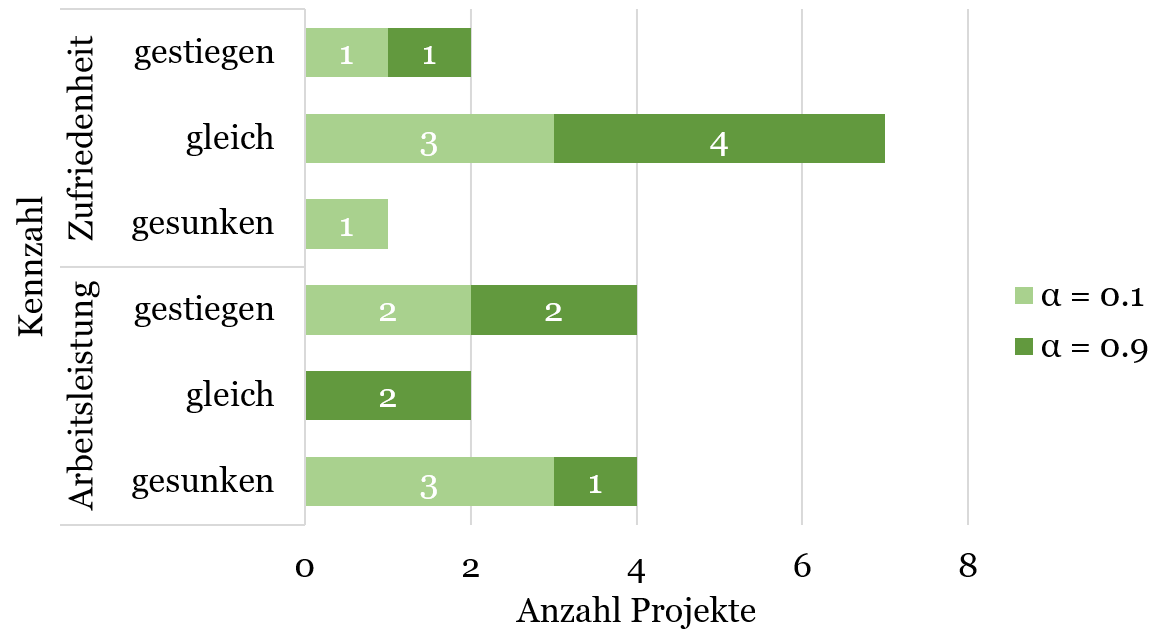
\includegraphics[width=0.95\textwidth]{gfx/verhaeltnis-z-a-projekte-edge-cases.png}
	\caption[Veränderung von Zufriedenheit und Arbeitsleistung der Mitarbeiter von unilateralem zu bilateralem Algorithmus für Grenzfälle von $\alpha$]{Veränderung von Zufriedenheit und Arbeitsleistung der Mitarbeiter von unilateralem zu bilateralem Algorithmus für Grenzfälle von $\alpha$}
	\label{fig:diskussion:abb1}
\end{figure}

Die Abbildung stellt die Veränderung der Zufriedenheit und der Arbeitsleistung von unilateralem zu bilateralem Algorithmus in Abhängigkeit der Grenzfälle für $\alpha$ dar.
Darin ist zu erkennen, bei wie vielen Projekten eine Kennzahl durch den bilateralen Algorithmus im Vergleich zum unilateralen Algorithmus gestiegen, gesunken oder gleich geblieben ist.
Auffällig ist, dass entgegen der Erwartungen eine marginale Gewichtung der Fähigkeiten ($\alpha$ = 0.1) in zwei von fünf Projekten sogar zu einer Steigerung der Arbeitsleistung der empfohlenen Mitarbeiter führte.
Des Weiteren ist auffällig, dass eine Berücksichtigung der Präferenzen ($\alpha$ = 0.9), wenn auch geringfügig, in einem der fünf Projekte zu einem Rückgang der Zufriedenheit unter den Angestellten führte.
Es wird deutlich, dass auch für Grenzfälle des Gewichts $\alpha$ kein kausaler Zusammenhang zwischen der Höhe des Gewichts und der Auswirkung auf die Zufriedenheit bzw. die Arbeitsleistung in den Daten zu bestehen scheint.
Eine Vermutung ist, dass die geringe Bedeutung der Gewichtung in dem Experiment unter anderem darauf zurückzuführen ist, dass viele Mitarbeiter die Fähigkeiten präferieren, die sie auch beherrschen (Vgl. Abbildung \ref{fig:ergebnisse:abb1}).
Folglich führt eine geringe Gewichtung der Fähigkeiten und eine damit einhergehende hohe Gewichtung der Präferenzen nicht umgehend zu einer geringen Arbeitsleistung.
Umgekehrt führt eine hohe Gewichtung der Fähigkeiten und eine damit einhergehende niedrige Gewichtung der Präferenzen nicht zwangsläufig zu einer geringeren Zufriedenheit.

% - integration der negativen präferenzen diskutieren
Abschließend wurde anhand der Forschungsergebnisse von \textcite[S. 1ff.]{link:booklet} angenommen, dass eine zusätzliche Berücksichtigung negativer Präferenzen bei der Zuordnung von Personen zu Projekten zu robusteren Ergebnissen führt.
Daher wurden in Anlehnung an das Vorgehen von \textcite[S. 269ff.]{pizzato:2:inproceedings} negative Präferenzen in den bilateralen Algorithmus integriert.
Wie eingangs angeführt, haben die Ergebnisse des Experiments gezeigt, dass der bilaterale Algorithmus in 2 von 25 Fällen eine Verschlechterung der Zufriedenheit und in 3 von 25 Fällen einen Rückgang der zu erwartenden Arbeitsleistung der Mitarbeiter bewirkte.
Trotz einer Berücksichtigung der negativen Präferenzen der Mitarbeiter konnte in dem Experiment folglich keine durchgängige Steigerung der Zufriedenheit und Arbeitsleistung der Angestellten erzielt werden. 
Um ein bilaterales Empfehlungssystem robust gegen Ausreißer zu gestalten, reicht eine zusätzliche Berücksichtigung negativer Präferenzen bei der Empfehlungserstellung folglich nicht aus.
Zusätzlich wird davon ausgegangen, dass auch bei den negativen Präferenzen spezifische Fähigkeiten für einen Mitarbeiter dominieren und demnach dessen Zufriedenheit stärker beeinflussen als andere.

% Darüber hinaus wird angenommen, dass die geringe Bedeutung der Gewichtung auch darauf zurückzuführen ist, dass viele Mitarbeitende die Fähigkeiten präferieren, die sie auch beherrschen.
% Folglich führt eine geringe Gewichtung der Fähigkeiten und eine damit einhergehende hohe Gewichtung der Präferenzen nicht umgehend zu einer geringen Arbeitsleistung.
% Umgekehrt führt eine hohe Gewichtung der Fähigkeiten und eine damit einhergehende niedrige Gewichtung der Präferenzen nicht zwangsläufig zu einer geringeren Zufriedenheit.

\section{Beschränkungen der Forschung}
Begrenzungen der Forschung ergaben sich beim Durchführen der Befragung der Manager.
Es wird angenommen, dass der Umfang der Befragung die Antworten der Manager beeinträchtigt haben.
So wurde bei Betrachtung der Antwortzeiten der Manager deutlich, dass einige Manager nur wenige Minuten für das Ausfüllen der Umfrage aufwendeten, was für ein intuitiveres Entscheidungsverhalten spricht.
Zugleich investierte der Manager mit der längsten Antwortzeit knapp 45 Minuten für das Ausfüllen der Befragung, was ein detaillierteres Betrachten der einzelnen Mitarbeiter und deren Fähigkeiten bzw. Präferenzen vermuten lässt.

% Weiter konnte bei Auswertung der Antworten der Manager festgestellt werden, dass in einigen Projekten große Diskrepanzen zwischen den von den Managern angegebenen Mitarbeitenden mit zu erwartend hoher Arbeitsleistung zu erkennen waren (Vgl. Abbildung \ref{fig:ergebnisse:abb5}).
% Obwohl den Managern lediglich die Namen der Mitarbeitenden, deren Fähigkeiten und Präferenzen vorlagen, konnten die Entscheidungen der Manager in einigen Fällen nicht anhand der vorliegenden Daten erklärt werden.
% Es wird davon ausgegangen, dass neben den Fähigkeiten und Präferenzen externe Faktoren die Entscheidungsfindung der Manager beeinflusst haben.
% Um den eindeutigen Einfluss der Fähigkeiten und Präferenzen auf die zu erwartende Arbeitsleistung eines Mitarbeitenden seitens der Manager zu ermitteln, gilt es diese Faktoren in zukünftigen Studien zu berücksichtigen.

Weiter ließ die Auswertung der Mitarbeiterbefragung vermuten, dass die Gestaltung der Beispielprojekte einen Einfluss auf die Zufriedenheit der Befragten hatte.
Da der Großteil der Beispielprojekte maßgeblich an das Anforderungsprofil eines Entwicklers gerichtet war, wird angenommen, dass Mitarbeiter anderer Fachbereiche ihre Zufriedenheit tendenziell bei Projekten höher bewerteten, die ihnen bekannte Fähigkeiten aufwiesen, auch wenn sie diese nicht präferierten.
Es wird angenommen, dass dadurch in Teilen die Aussagekraft hinsichtlich der Zufriedenheit der Mitarbeiter mit den Projekten beeinträchtigt wurde.
% - managerbefragung anführen, zu wenig zeit genommen, liegen weit auseinander etc.
% - mitarbeitendenbefragung war sehr spezifisch für entwickler -> bspw. agile coach haben dann höhere zufriedenheit bei projekt 3, obwohl sonst viele dinge nicht stimmen

In den theoretischen Grundlagen in Kapitel \ref{ch:erweiterungen} wurden verschiedene Möglichkeiten für die Berücksichtigung mehrerer Kriterien bei der Empfehlungserstellung vorgestellt.
Das Ziel dieser Arbeit war nicht, die Auswirkungen der verschiedenen Möglichkeiten miteinander zu vergleichen, sondern einen Überblick über die verschiedenen Verfahren zu bieten und einen für den Anwendungsfall sinnvollen Ansatz zu implementieren.

Darüber hinaus war es nicht Inhalt dieser Arbeit den eindeutigen Einfluss der Berücksichtigung negativer Präferenzen auf die Zufriedenheit und Arbeitsleistung der Mitarbeiter zu bestimmen.
Um eine eindeutige Aussage über die Auswirkung der Berücksichtigung negativer Präferenzen auf Zufriedenheit und Arbeitsleistung der Mitarbeiter bei der Zuordnung zu Projekten treffen zu können, sollte die Berücksichtigung der negativen Präferenzen in einer weiterführenden Fallstudie isoliert betrachtet werden.

\section{Empfehlungen für weiterführende Forschung}
Insgesamt lassen die Ergebnisse der Auswirkungen des bilateralen Algorithmus auf die Zufriedenheit und die Arbeitsleistung der Mitarbeiter die Vermutung zu, dass eine Berücksichtigung der Präferenzen grundsätzlich vorteilhaft ist.
Dabei scheint es eine geringfügigere Rolle zu spielen, welches Gewicht den Präferenzen zukommt.
Die Erwartung ist, dass die Auswirkungen der Berücksichtigung der Präferenzen vorallem dann entscheidend ist, wenn die beherrschten und präferierten Fähigkeiten der Angestellten weiter auseinanderliegen.
Um den Effekt der Gewichte auf die Zufriedenheit und Arbeitsleistung genauer zu untersuchen, wird daher empfohlen eine weitere Studie durchzuführen, die auf solchen Daten basiert.
Diese Daten können dann herangezogen werden, um eine optimale Gewichtung der Fähigkeiten und Präferenzen bei der Zuordnung der Mitarbeiter zu Projekten anhand des vorgestellten Verfahrens in Kapitel \ref{ch:methodik} zu ermitteln.
Eine größere Datenmenge als Ausgangsbasis würde zusätzlich zu der Robustheit des Algorithmus unter Einsatz des Gewichts beitragen, da erwartet wird, dass sich das Gewicht über eine Vielzahl an Daten hinweg in einem bestimmten Bereich einpendelt.

Darüber hinaus konnte im Rahmen der Arbeit festgestellt werden, dass sowohl die Zufriedenheit als auch die Arbeitsleistung der Mitarbeiter durch weitere unbekannte Kriterien beeinflusst werden.
Um den eindeutigen Einfluss der Fähigkeiten und Präferenzen auf die Zufriedenheit und die erwartende Arbeitsleistung eines Mitarbeiters seitens der Manager zu ermitteln, gilt es, diese Kriterien in weiterführenden Forschungen zu identifizieren.
% Eine Empfehlung für weitere Forschungen ist daher, diese Kriterien zu identifizieren.
Eine mögliche Vorgehensweise wäre hier das Durchführen von Experteninterviews unter den Managern und Mitarbeitern.
Die Kriterien sollten dann anhand einer der vorgestellten Methoden in Kapitel \ref{ch:erweiterungen:loesungen} als zusätzliche Kriterien in das multi-kriterielle Empfehlungssystem integriert werden.

In Kapitel \ref{ch:erweiterungen:einführung} wurde angeführt, dass multi-kriterielle Problemstellungen in Organisationen der Kategorie der Entscheidungsprobleme zugeordnet werden können.
Auch die Zuordnung von Mitarbeitern zu Projekten anhand verschiedener Kriterien kann folglich als Entscheidungsproblem betrachtet werden.
Eine Frage für weiterführende Arbeiten stellt dar, wieviel dieser Entscheidung einem System und wieviel dem Entscheidungsträger bzw. den Entscheidungsträgern überlassen werden soll.
Hinsichtlich der Intergration der Präferenzen in die Empfehlungserstellung wäre denkbar, die Berücksichtigung der Präferenzen an den bzw. die Entscheidungsträger auszulagern.
Dies könnte beispielsweise in Form einer grafischen Oberfläche gestaltet werden, in der Entscheidungsträger die Möglichkeit haben selbstständig einzustellen, wie sehr sie die Präferenzen der Mitarbeiter bei der Zuordnung zu Projekten berücksichtigen wollen.

% interpretation der gewählten art der integration -> gewichtete summe anstatt von harmonischem Mittel zb


% Abgleich Präferenzen angeforderte Projektpositionen:
% Ein detaillierter Abgleich der Mitarbeitenden, die angaben mit Projekt 5 zufrieden zu sein, mit den Mitarbeitenden, die eine hohe Übereinstimmung aufwiesen (> 80 Prozent) zeigte, dass lediglich 5 dieser 13 Mitarbeitenden auch angaben, mit dem Projekt zufrieden zu sein.
% Weiter ist zu erkennen, dass Projekt 4 zwar bei der Befragung der Zufriedenheit die höchste Anzahl an zufriedenen Mitarbeitenden aufwies ($\approx$ 30 Befragte), in der Übereinstimmung der Präferenzen jedoch im Vergleich am zweitwenigsten Mitarbeitende eine Übereinstimmung über 40 Prozent aufwiesen.
% Darüber hinaus liegt die Anzahl an Mitarbeitenden mit einer Übereinstimmung der Präferenzen unter 20 Prozent\footnote{inkl.} bei Projekt 4 mit 23 Befragten mit Abstand am höchsten.
% Hier wieder bei diskussion die  schwankung erklären -> annahme, dass das mit der ANzahl der angeforderten Projektpositionen zusammenhängt!

% Argumentation:
% \begin{itemize}
%     \item Zufriedenheit zu integrieren ist auf jeden Fall gut -> daher ergebnisse besser
%     \item Wie dann gewichtet wird scheint weniger eine Rolle zu spielen -> sehr schwankende Ergebnisse
%     \item Die geringe Bedeutung der Gewichtung kann auch darauf zurückzuführen sein, dass viele Mitarbeitende auch das präferieren, was sie können (daher ist die Diskrepanz zwischen hohem und kleinen gewicht nicht so groß) -> überprüfen!!
%     \item Haupterkenntnis ist also, dass es wichtig ist die Zufriedenheit zu berücksichtigen, Gewicht an sich aber kaum eine Rolle gespiel that, hauptsache die Präferenzen sind dabei
%     \item Die Präferenzen ist dann das was den unterschied macht zwischen "Mitarbeitender passt" und "Mitarbeitender passt gut"
%     \item Viele unbekannte Einflussfaktoren auf die Zufriedenheit: Gewichtung der einzelnen Präferenzen für einen Mitarbeitenden, andere Projekte die zur Auswahl stehen
%     \item Unbekannte Einflussfaktoren auf die Arbeitsleistung: welche Fähigkeiten einem Mitarbeitendem fehlen spielt eine entscheidende rolle -> kann er diese schnell erlernen oder nicht?
%     \item Next steps: Experteninterviews um zu identifizieren, was das kernproblem des bestehenden algorithmus ist und dann kriterium mit aufnehmen anhand einer der vorgestellten maßnahmen
%     \item perspektivisch auch die Präferenzen integrieren, aber geringere Bedeutung als andere Kriterien (Verfügbarkeit, Vollständigkeit und Aktualität der Daten, Teamzugehörigkeit)
%     \item Wichtige überlegung: problem der auswahl mitarbeitender für projekte ist entscheidungsproblem -> Frage, wieviel man dem system übergibt und was man den Managern noch an Entscheidung überlässt (bspw. Zufriedenheit als slider)
% \end{itemize}

%Ein Vergleich der Veränderungen bei beiden Kennzahlen zeigt zudem, dass die Zufriedenheit im Verhältnis zu der erwarteten Arbeitsleistung in mehr Fällen gestiegen ist.
% Zugleich führte der bilaterale Algorithmus in zwei Fällen zu einer Verschlechterung der zu erwarteten Arbeitsleistung und in einem Fall zu einer Verschlechterung der Zufriedenheit.

% Bei den Gewichten: wenn sich sowohl alpha als auch mitarbeitende ändern dann verändert sich zu viel input -> ob ein mitarbeitender dann in liste ist oder nicht ist zu ausschlaggebend
% wenn alle mitarbeitende gleich bleiben und nur alpha sich verändert kommen trotzdem komische werte raus :D
% dass bei 4 der 5 verschiedenen gewichte eine steigerung erzielt werden konnte deutet eher darauf hin, dass die gewichtung hier nicht ausschlaggebend war. dies spricht auch dafür, dass bei demselben gewicht die zufriedenheit bei manchen gewichten sowohl gestiegen als auch gesunken ist 
% -> hier auch ergebnisse über alle mitarbeitenden hinweg anführen für die edge cases 0,1 und 0,9 und zeigen, wie es sich da verhält
% Daraus geht hervor, dass keines der Gewichte eindeutig zu einer Verbesserung oder einer Verschlechterung im Vergleich zum unilateralen Algorithmus geführt hat.

% Was offen bleibt: Endlichkeit von Elementen -> Wie MA zuordnen, dass nicht immer ein MA, der alles kann für alles Projekte vorgeschlagen wird? (Berücksichtigung der Verfügbarkeit als Slider)
% Berücksichtigung von Teamzugehörigkeit

% Nutzerbasierte (in unserem Fall elementbasiert, da MA die Elemente sind) Gewichtung -> Gewichtung der Präferenzen im Verhältnis zu Fähigkeiten von MA zu MA unterschiedlich wichtig

\shorthandon{"}